\section{実験}\label{chap:exp}

本節では,4節で説明した根付き全域森探索問題の各符号化の評価と,
5節で説明した遷移問題を解く各手法の評価のために行った実験に
ついて説明する.

まず,根付き全域森探索問題の符号化の評価実験について述べる.
実験は,提案した基本符号化(コード\ref{code:srf1.lp})と改良符号化
(コード\ref{code:srf2.lp})を用いて各問題を符号化し,1問あたりの制限
時間を1時間として\clingo で実行し,解いた問題数,各問題の実行CPU
時間と制約数を集計する.なお,\clingo のバージョンは 5.4.0,
ソルバーオプションとして\textit{trendy}を使用した.実験環境は,
Mac mini,3.2 GHz Intel Core i7,64GB メモリである.

なお,ベンチマーク問題として,DNET\footnote{\url{https://github.com/takemaru/dnet}}
で公開されている配電網モデルからトポロジ制約のみを抽出した3問と,
Graph Coloring and its Generalization\footnote{\url{http://mat.tepper.cmu.edu/COLOR04/}}
で公開されているグラフ彩色問題127問中,辺の数が50000以下である
非連結成分を含まない無向グラフ82問を用いた.また,グラフ彩色問題
については,ノードのうち1/5個をランダムに根として与えた.これらの
計85問の問題のノードの数は11〜1406,辺の数は16〜49629,根の数は1〜281である.

実験結果として,各符号化の性能を比較するためにカクタスプロットに
よる比較を図\ref{fig:cactus}に示す.カクタスプロットは,縦軸が
各問題を解くまでのCPU時間を表し,横軸が解けた問題数を表す.グラフが
下に寄るほど多くの問題を高速に解いていることを示し,右に寄るほど
制限時間内に多くのベンチマーク問題を解くことが可能であることを意味
するので,右下に行くほど符号化の性能が良いとされる.

%%%%%%%%%%%%%%%%%%%%%%%%%%%%%%%%%%%%%%%%
% 貼れない !!!!!!!!!!!!!!!!!!!!!!11
%%%%%%%%%%%%%%%%%%%%%%%%%%%%%%
\begin{figure}[htbp]
 \centering
 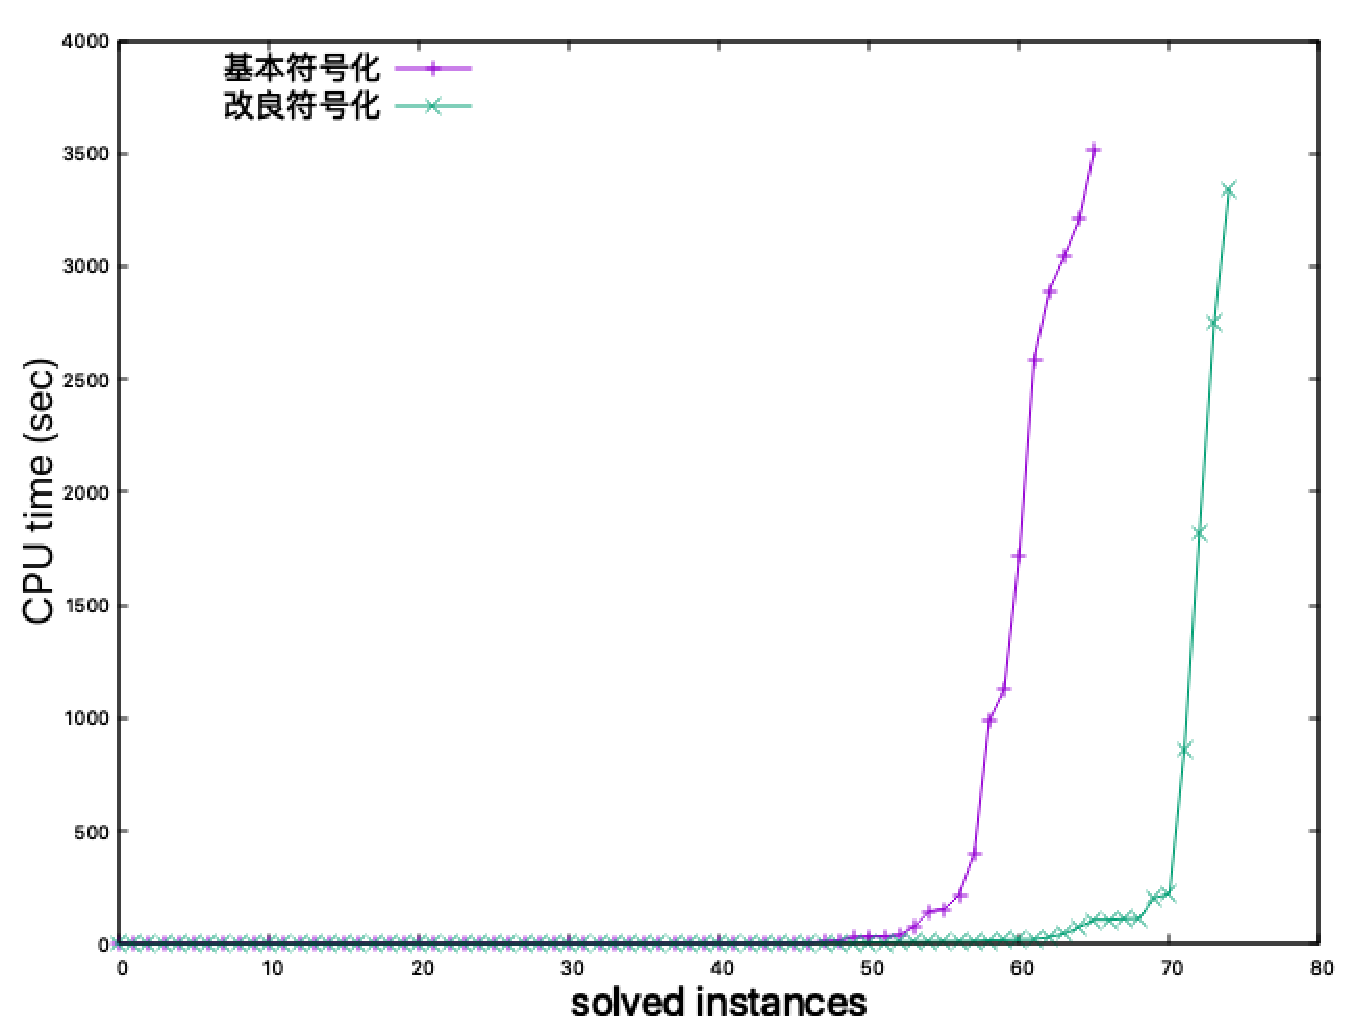
\includegraphics[scale=0.3]{fig/cactus.eps}
 \caption{比較結果: カクタスプロット} 
 \label{fig:cactus}
\end{figure}
%%%%%%%%%%%%%%%%%%%%%%%%%%%%%%

結果では,改良符号化は基本符号化と比較して,より多くの問題を高速に
解いていることを示した.したがって改良符号化のほうが性能が良いこと
がいえる.

続いて,実際に各符号化が解いた問題について,グラフの辺の数で問題を
分類して比較したものを表\ref{table:kibo}に示す.表中の太字は,解けた
問題数を比較して多い方,または同数であることを表している.

%%%%%%%%%%%%%%%%%%%%%%%%%%%%%%
\begin{table}[htbp]
  \caption{比較結果: 解けた問題数(問)}
  \label{table:kibo}
  \centering
 \begin{tabular}[t]{c|c|c|c}
  \noalign{\hrule height 1pt}
  辺の数 & 問題数 & 基本符号化 & 改良符号化 \\
  \noalign{\hrule height 1pt}
%%%%%%%%
  1 ~ 1000 & 30 & \textbf{30} & \textbf{30} \\
  \hline
  1001 ~ 4000 & 20 & \textbf{20} & \textbf{20} \\
  \hline
  4001 ~ 7000 & 11 & 9 & \textbf{10} \\
  \hline
  7001 ~ 10000 & 8 & 4 & \textbf{6} \\
  \hline
  10001 ~ 20000 & 9 & 2 & \textbf{5} \\
  \hline
  20001 ~ 30000 & 2 & 1 & \textbf{2} \\
  \hline
  30001 ~ 40000 & 1 & 0 & 0 \\
  \hline
  40001 ~ 50000 & 4 & 0 & \textbf{2} \\
%%%%%%%% 合計
  \noalign{\hrule height 1pt}
  計 & 85 & 66 & \textbf{75} \\
  \noalign{\hrule height 1pt}
 \end{tabular}
\end{table}
%%%%%%%%%%%%%%%%%%%%%%%%%%%%%%

結果から,辺の数が少ない問題では符号化による解けた問題数の差は
大きく見られないが,辺の数が10,000を超える問題では,改良符号化
の方が基本符号化よりも多くの問題を解いたことを示した.また,改良
符号化は辺の数が40,000を超えるような大規模の問題に対しても,解を
求めることに成功した.これらの結果から,4.2節で述べた改良符号化の
特長である,根付き連結制約を符号化した際の制約数が少なく抑えられる
ことが拡張性の高さに有効であるといえる.

次に,遷移問題に関して行った実験について述べる.
実験は,外部プログラムを利用する手法(コード\ref{code:roop})と,
\clingo のライブラリを利用する手法(コード\ref{code:incmode})の比較を
行った.各手法について,各問題を解くまでにかかったCPU時間を比較する.
実験に用いたASPソルバー・環境は,先程説明したものと同じものを用いた.

ベンチマーク問題については,実用規模の配電網モデル(ノード数:432,根ノード数:72)
からできる実行可能解からランダムに初期状態として5つ,目的状態として6つを
それぞれ抽出し,それらを組み合わせた計30問を用いた.

実験を行った結果を表\ref{table:trans}に示す.なお,表中の比率は,外部プログラム
での探索時間を1としたときのライブラリによる探索時間を示す.今回行った実験では,
すべての問題についてライブラリによる探索のほうが高速に解いていることがわかる.
また,今回行った実験では探索回数が11回,すなわち遷移回数が10回の問題についても
解を求めることにも成功している.比率について平均をとると$32.8\%$となり,$67.2\%$
もの探索時間の短縮ができていることが確認できる.したがって\clingo のライブラリを
利用することでオーバヘッドの短縮及び部分的な学習節の利用が有効に働いていると
いえる.

\begin{table*}[htbp]
 \centering
 \caption{実験結果}
 \label{table:trans}
 \begin{tabular}{c|r|r|r|r}  
 \noalign{\hrule height 1pt}
 問題名 & \multicolumn{1}{|c|}{ステップ長$t$} & \multicolumn{1}{|c|}{外部(sec)} 
		 & \multicolumn{1}{|c|}{ライブラリ(sec)} & \multicolumn{1}{|c}{比率(\%)} \\
 \noalign{\hrule height 1pt}
s1\_g60 & 8 & 50.098 & 25.659 & 51.2 \\
s1\_g70 & 8 & 47.177 & 24.981 & 53.0 \\
s1\_g80 & 8 & 43.193 & 15.852 & 36.7 \\
s1\_g90 & 8 & 48.984 & 22.983 & 46.9 \\
s1\_g100 & 6 & 20.964 & 4.709 & 22.5 \\
\hline
s10\_g60 & 6 & 21.947 & 5.132 & 23.4 \\
s10\_g70 & 8 & 43.840 & 16.290 & 37.2 \\
s10\_g80 & 6 & 21.156 & 4.887 & 23.1 \\
s10\_g90 & 6 & 21.276 & 5.324 & 25.0 \\
s10\_g100 & 8 & 45.704 & 17.697 & 38.7 \\
\hline
s20\_g60 & 6 & 21.202 & 4.973 & 23.5 \\
s20\_g70 & 4 & 9.890 & 2.699 & 27.3 \\
s20\_g80 & 8 & 48.473 & 16.335 & 33.7 \\
s20\_g90 & 10 & 107.938 & 64.441 & 59.7 \\
s20\_g100 & 8 & 48.473 & 17.894 & 36.9 \\
\hline
s30\_g60 & 6 & 21.189 & 5.287 & 25.0 \\
s30\_g70 & 4 & 9.901 & 2.735 & 27.6 \\
s30\_g80 & 6 & 21.884 & 5.223 & 23.9 \\
s30\_g90 & 4 & 9.979 & 2.658 & 26.6 \\
s30\_g100 & 8 & 50.344 & 18.845 & 37.4 \\
\hline
s40\_g60 & 8 & 44.637 & 14.254 & 31.9 \\
s40\_g70 & 6 & 21.334 & 4.795 & 22.5 \\
s40\_g80 & 8 & 45.202 & 14.099 & 31.2 \\
s40\_g90 & 6 & 21.710 & 5.119 & 23.6 \\
s40\_g100 & 6 & 21.299 & 5.666 & 26.6 \\
\hline
s50\_g60 & 4 & 10.021 & 2.726 & 27.2 \\
s50\_g70 & 6 & 21.291 & 4.718 & 22.2 \\
s50\_g80 & 6 & 21.163 & 6.503 & 30.7 \\
s50\_g90 & 10 & 108.299 & 65.352 & 60.3 \\
s50\_g100 & 4 & 9.934 & 2.700 & 27.2 \\
 \noalign{\hrule height 1pt}
\multicolumn{4}{c|}{平均比率(\%)} & 32.8 \\
 \noalign{\hrule height 1pt}
\end{tabular}

\end{table*}

